\section{Discussion}
In this section we demonstrate our algorithm by an example. Reference grammar $G$ is the following:\\
(0) start\_rule ::= s \\
(1) s ::= LBR s RBR s\\
(2) s ::= $\varepsilon$ \\

Consider the following input FA constructed by tokenization of some regular approximated string-embedded code~\ref{faApprox}.
% \begin{figure}[!ht]
%    \subfloat[First sub-figure\label{subfig-1:dummy}]{%
%      \includegraphics[scale=0.3]{dot/in3.eps}
%    }
%    \hfill
%    \subfloat[First sub-figure\label{subfig-2:dummy}]{%
%      \includegraphics[scale=0.3]{dot/out3.eps}
%    }
%    \caption{Dummy figure}
%    \label{fig:dummy}
%  \end{figure}
\begin{figure}
    \begin{center}
        \includegraphics[scale=0.5]{dot/in3.eps}
    \end{center}
    \caption{$A_1$ -- input for our algorithm: regular approximation for string-embedded code after tokenization} 
    \label{faApprox}
\end{figure}

As you can see, some of the sentences from the language described by FA $A_1$ do not belong to the reference language $L(G)$.
For example let $s$ = \verb|LBR LBR RBR| (``\verb|(()|'' before tokenization): $s \in L(A_1)$ but $s \notin L(G)$.
The algorithm ignores such erroneous strings and constructs SPPF which contains derivatiom trees for all sentences $s \in L(A_1)$ such that $s \in L(G)$.
The SPPF constructed is presented in figure~\ref{resultSPPF}.
\begin{figure}
    \begin{center}
        \includegraphics[scale=0.3]{dot/out3.eps}
    \end{center}
    \caption{SPPF for input FA presented in figure~\ref{faApprox}}
    \label{resultSPPF}
\end{figure}

Presented algoritm report failure only if $L_a \cap L_r = \emptyset$. It might be considered a problem, but there are two possible ways to overcome such limitation. 
As far as language inclusion problem is decidable (in the constraints of our algorithm), first, all the erroneous strings could be found with proper algorithm, 
after which forest could be constructed for the subset of correct strings. 
The second way is to modify algorithm so that besides parse forest construction for all correct strings belonging to $L_a$ 
it reports all existent incorrect strings.

Known works does not provide full theoretical estimation for string-embedded languages parsing complexity in depends on input, so it is open question for future reserach.

Described algorithm produce SPPF which is utilized for trees extraction and sematic calculation in original RNGLR. Semantic actions may be specified with attributed grammar.
Semantic processing and transformations for string-embedded languages can find its application in migration to more principal aproaches of dynamic code generation, as proposed in~\cite{EvalToStaged}.
We also can use this approach to specify semantic, but, unfortunately, termination and correctness of semantic calcualtion and transformation is a topic for further research 
as in our case SPPF contains cycles which cannot be elaminated. 

% Context-free approximation processing?
% Implementation in IDE?  
